\documentclass[tikz,border=2pt]{standalone}
\usepackage{amsmath,amssymb}
\usepackage{pgfplots}
\pgfplotsset{compat=1.18}
\usetikzlibrary{arrows.meta}
\begin{document}
% G/G/1 departure scv approximation C_d^2 = (1-rho^2) C_a^2 + rho^2 C_s^2 with C_a^2 = 2, C_s^2 = 1/2,
% i.e. C_d^2 = 2 - 1.5 rho^2; it moves from C_a^2 at rho = 0 to C_s^2 at rho = 1; rho = 2/3 gives 4/3.
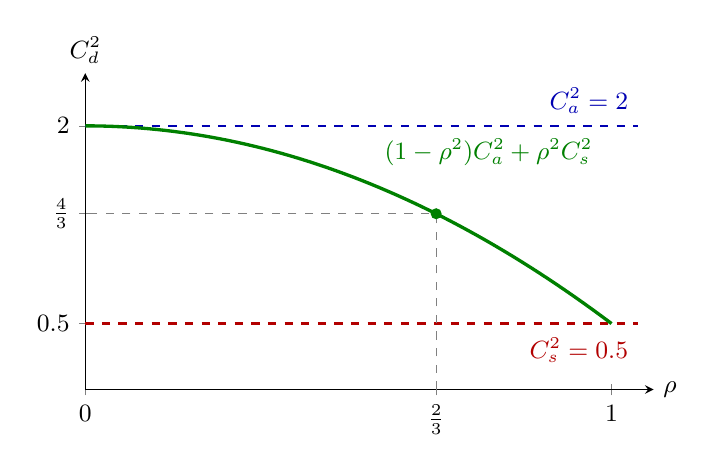
\begin{tikzpicture}[font=\small, >={Latex[length=2mm]}]
  \begin{axis}[
    axis lines=left, xmin=0, xmax=1.08, ymin=0, ymax=2.4,
    xtick={0,0.6667,1}, xticklabels={$0$,$\tfrac{2}{3}$,$1$},
    ytick={0.5,1.3333,2}, yticklabels={$0.5$,$\tfrac{4}{3}$,$2$},
    xlabel={$\rho$}, ylabel={$C_d^2$},
    xlabel style={at={(axis description cs:1,0)}, anchor=west},
    ylabel style={rotate=-90, at={(axis description cs:0,1)}, anchor=south},
    width=8.8cm, height=5.6cm, clip=false]
    \draw[blue!70!black, thick, dashed] (axis cs:0,2) -- (axis cs:1.05,2);
    \node[blue!70!black, anchor=south east] at (axis cs:1.05,2.02) {$C_a^2=2$};
    \draw[red!70!black, thick, dashed] (axis cs:0,0.5) -- (axis cs:1.05,0.5);
    \node[red!70!black, anchor=north east] at (axis cs:1.05,0.47) {$C_s^2=0.5$};
    \addplot[green!50!black, very thick, domain=0:1, samples=60] {2 - 1.5*x^2};
    \node[green!50!black, anchor=west] at (axis cs:0.55,1.8) {$(1-\rho^2)C_a^2+\rho^2C_s^2$};
    \draw[gray, thin, dashed] (axis cs:0.6667,0) -- (axis cs:0.6667,1.3333) -- (axis cs:0,1.3333);
    \fill[green!50!black] (axis cs:0.6667,1.3333) circle (2pt);
  \end{axis}
\end{tikzpicture}
\end{document}
